\documentclass{article}

\usepackage{graphicx}
\usepackage{listings, lstautogobble}
\usepackage{color}
\usepackage{hyperref}
\usepackage{float}

% paper margin
\usepackage{geometry}
\geometry{
	a4paper,
	total={170mm,257mm},
	left=14mm,
	right=14mm,
	top=14mm,
}

% multi-column
\usepackage{multicol}
\setlength{\columnsep}{1cm}

% color definition
\definecolor{dkgreen}{rgb}{0,0.6,0}
\definecolor{gray}{rgb}{0.5,0.5,0.5}
\definecolor{mauve}{rgb}{0.58,0,0.82}

% listing
\lstset{frame=tb,
  language=C++,
  aboveskip=3mm,
  autogobble=true,
  belowskip=3mm,
  showstringspaces=false,
  columns=flexible,
  basicstyle={\small\ttfamily},
  numbers=none,
  numberstyle=\tiny\color{gray},
  keywordstyle=\color{blue},
  commentstyle=\color{dkgreen},
  stringstyle=\color{mauve},
  breaklines=true,
  breakatwhitespace=true,
  tabsize=3
}

\begin{document}

	% paper title
    \title{
    	\textbf{SPH Fluid Simulation with Metaballs} \\
    	\large DD2323 Project Report \\}
   	\author{
		Alexander Hjelm\\
		\texttt{alhjelm@kth.se}
		\and
		Tsz Kin Chan\\
		\texttt{tkch@kth.se}
	}
    \date{\today}

    \maketitle
    
    \begin{multicols}{2}

    \section{Summary}
    %TODO: Write a summary
        In this project, we have rendered fluid-like 3D body in real time by using the Metaballs technique with the Marching Cubes rendering method. The project will cover the theory behind those technique, as well as outline our specific implementation in GLFW and GLSL. We could not render as many particles as we had hoped for, and in the end of the report we will discuss a few ideas for how to optimize both the particle model and the rendering, as well as present some alternative techniques that are more suitable for real time rendering purposes. Any reader that is interested in delving deeper will find the whole source code for this project available under the MIT license at this repository: \url{https://github.com/Alexander-Hjelm/metaballs-glfw}.
    
    \section{Introduction}
     
		Metaballs are soft, organic-looking 3D objects that appear to blob together when they are very close, and can be used to simulate dynamic fluids if using many particles on a large simulation domain. 
		The metaballs rendering technique was invented by Jim Blinn in the early 1980s, and has been a very common demo effect since the 1990s.
	
		The metaballs model is defined as a 3D isosurface, and can be rendered using the same methods that are common to isosurfaces. Most common methods for rendering metaballs are ray-tracing for still image and animations, and the marching cubes algorithm for real time.
		\cite{heckbert92}

	Using low-level graphics programming, we have programmed and rendered a real time, dynamic fluid using the metaballs with the marching cubes technique. The fluid particles use a basic physics model to collide with each other and the environment.

    This report will present the theory behind the metaballs rendering technique and show how it can be implemented as a real time simulation.
    
    \begin{figure}[H]
    	\centering
    	\begin{minipage}[b]{0.5\textwidth}
    		\centering
    		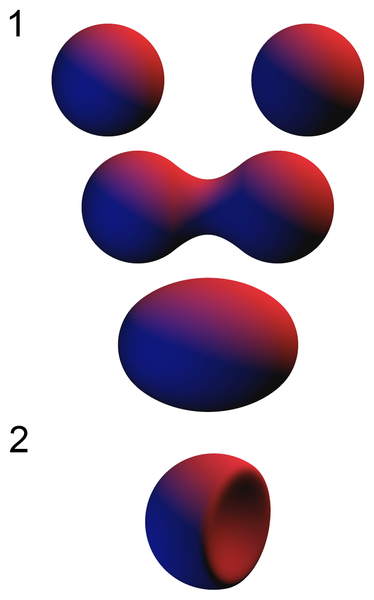
\includegraphics[width=0.3\textwidth]{img/metaballs-concept.png}
    		\caption{A conceptual visualisation of how metaballs work. 1 shows two metaballs gradually merging, and 2 shows the influence of a negative metaball on a positive metaball. \cite{wiki07}}
    		\label{fig:metaballs-concept}
    	\end{minipage}
    \end{figure}

    \section{Theory}

        \subsection{Metaball isosurface model}
            A metaball is an isosurface in 3D space. 
            Define a function $f(x,y,z)$, which takes as input a set of coordinates in 3D space, and returns a floating poing value that represents the influence of the function on that point.
            When we have such a function, we can sample it at even or random intervals to determine which points belong inside the surface and which belong outside it.
            This is simply a matter of comparing wether the influence at a point is greater than a fixed threshold or not.
            We can then use a number of different rendering techniques to create a presentation of this 3D surface, as we shall see in the next section.

            For now, let us look at the metaball surface model in particular. The most common isosurface fucntion for the metaball model is inverse quadratic:

            $[f(x,y,z) = 1.0 / (x^2 + y^2 + z^2)]$

            This function describes a field where each ball has an influence point with quadratic falloff.
            For any point $\vec{p}$ in 3D, and for any ball's position $\vec{b}$, the influence of that ball on the point $\vec{p}$ will be proporitonal to $|\vec{p} - \vec{b}|^2$.
            This function is also used to model the strength of electrical fields in electromagnetics, which is why we choose to label it as the metaball potetial field function.
            \cite{geiss00}

            If one were to draw the resulting field of a single metaball around the origin, it might look like figure 2, where the brightness of the color indicates the influence of the field at that point.
            
            A similar model for two metaballs, with their potential fields partially overlapping in different stages, is shown in figure 3.
            
            \begin{figure}[H]
            	\centering
            	\begin{minipage}[b]{0.2\textwidth}
            		\centering
            		
\includegraphics[width=\textwidth]{img/2d-potential.png}
            		\caption{A concept of the inverse square function in 2D}
		            \label{fig:2d-potential}
            	\end{minipage}
            \end{figure}
        
        	\begin{figure}[H]
        		\centering
            	\begin{minipage}[b]{0.4\textwidth}
            		
\includegraphics[width=\textwidth]{img/2d-potential-multi.png}
            		\caption{A concept of 2 metaballs in 2D. Every frame shows the two balls moving closer to each other.}
            		\label{fig:2d-potential-multi}
            	\end{minipage}
            \end{figure}

            As you can see, the area between the two balls becomes gradually lit up.
            The intersection between two potential fields becomes brighter as the two balls move closer, and at some point the center point between the balls will have a strength that is above our threshold. This effect will propagate outwards as the balls move closer, and we will use this later to make the balls appear as if they blob together in 3D.

        \subsection{Marching cubes}
			Marching cubes is a well-known algorithm for constructing a polygonal mesh of an isosurface form a given scalar field. It was first published in the 1987 SIGGRAPH by William E. Lorensen and Harvey E. Cline, and was highly adopted in medical visualization.
			
			This algorithm takes a scalar field as an input, and output a list of triangles representing the isosurface. It iterates through the scalar field and calculate all corresponding value for each neighboring vertices in a voxel. Then depending on whether the value of neighbor vertices fall in or out of the isolevel, a list of triangle are generated according to the configuration. Since there are 8 vertices in a voxel, there are a total of 256 configurations of polygon placement as shown in figure 4. By combining all triangles generated within the scalar field, we can obtain the approximated polygonal mesh as a whole. 
			
			\begin{figure}[H]
				\centering
				\begin{minipage}[b]{0.4\textwidth}
					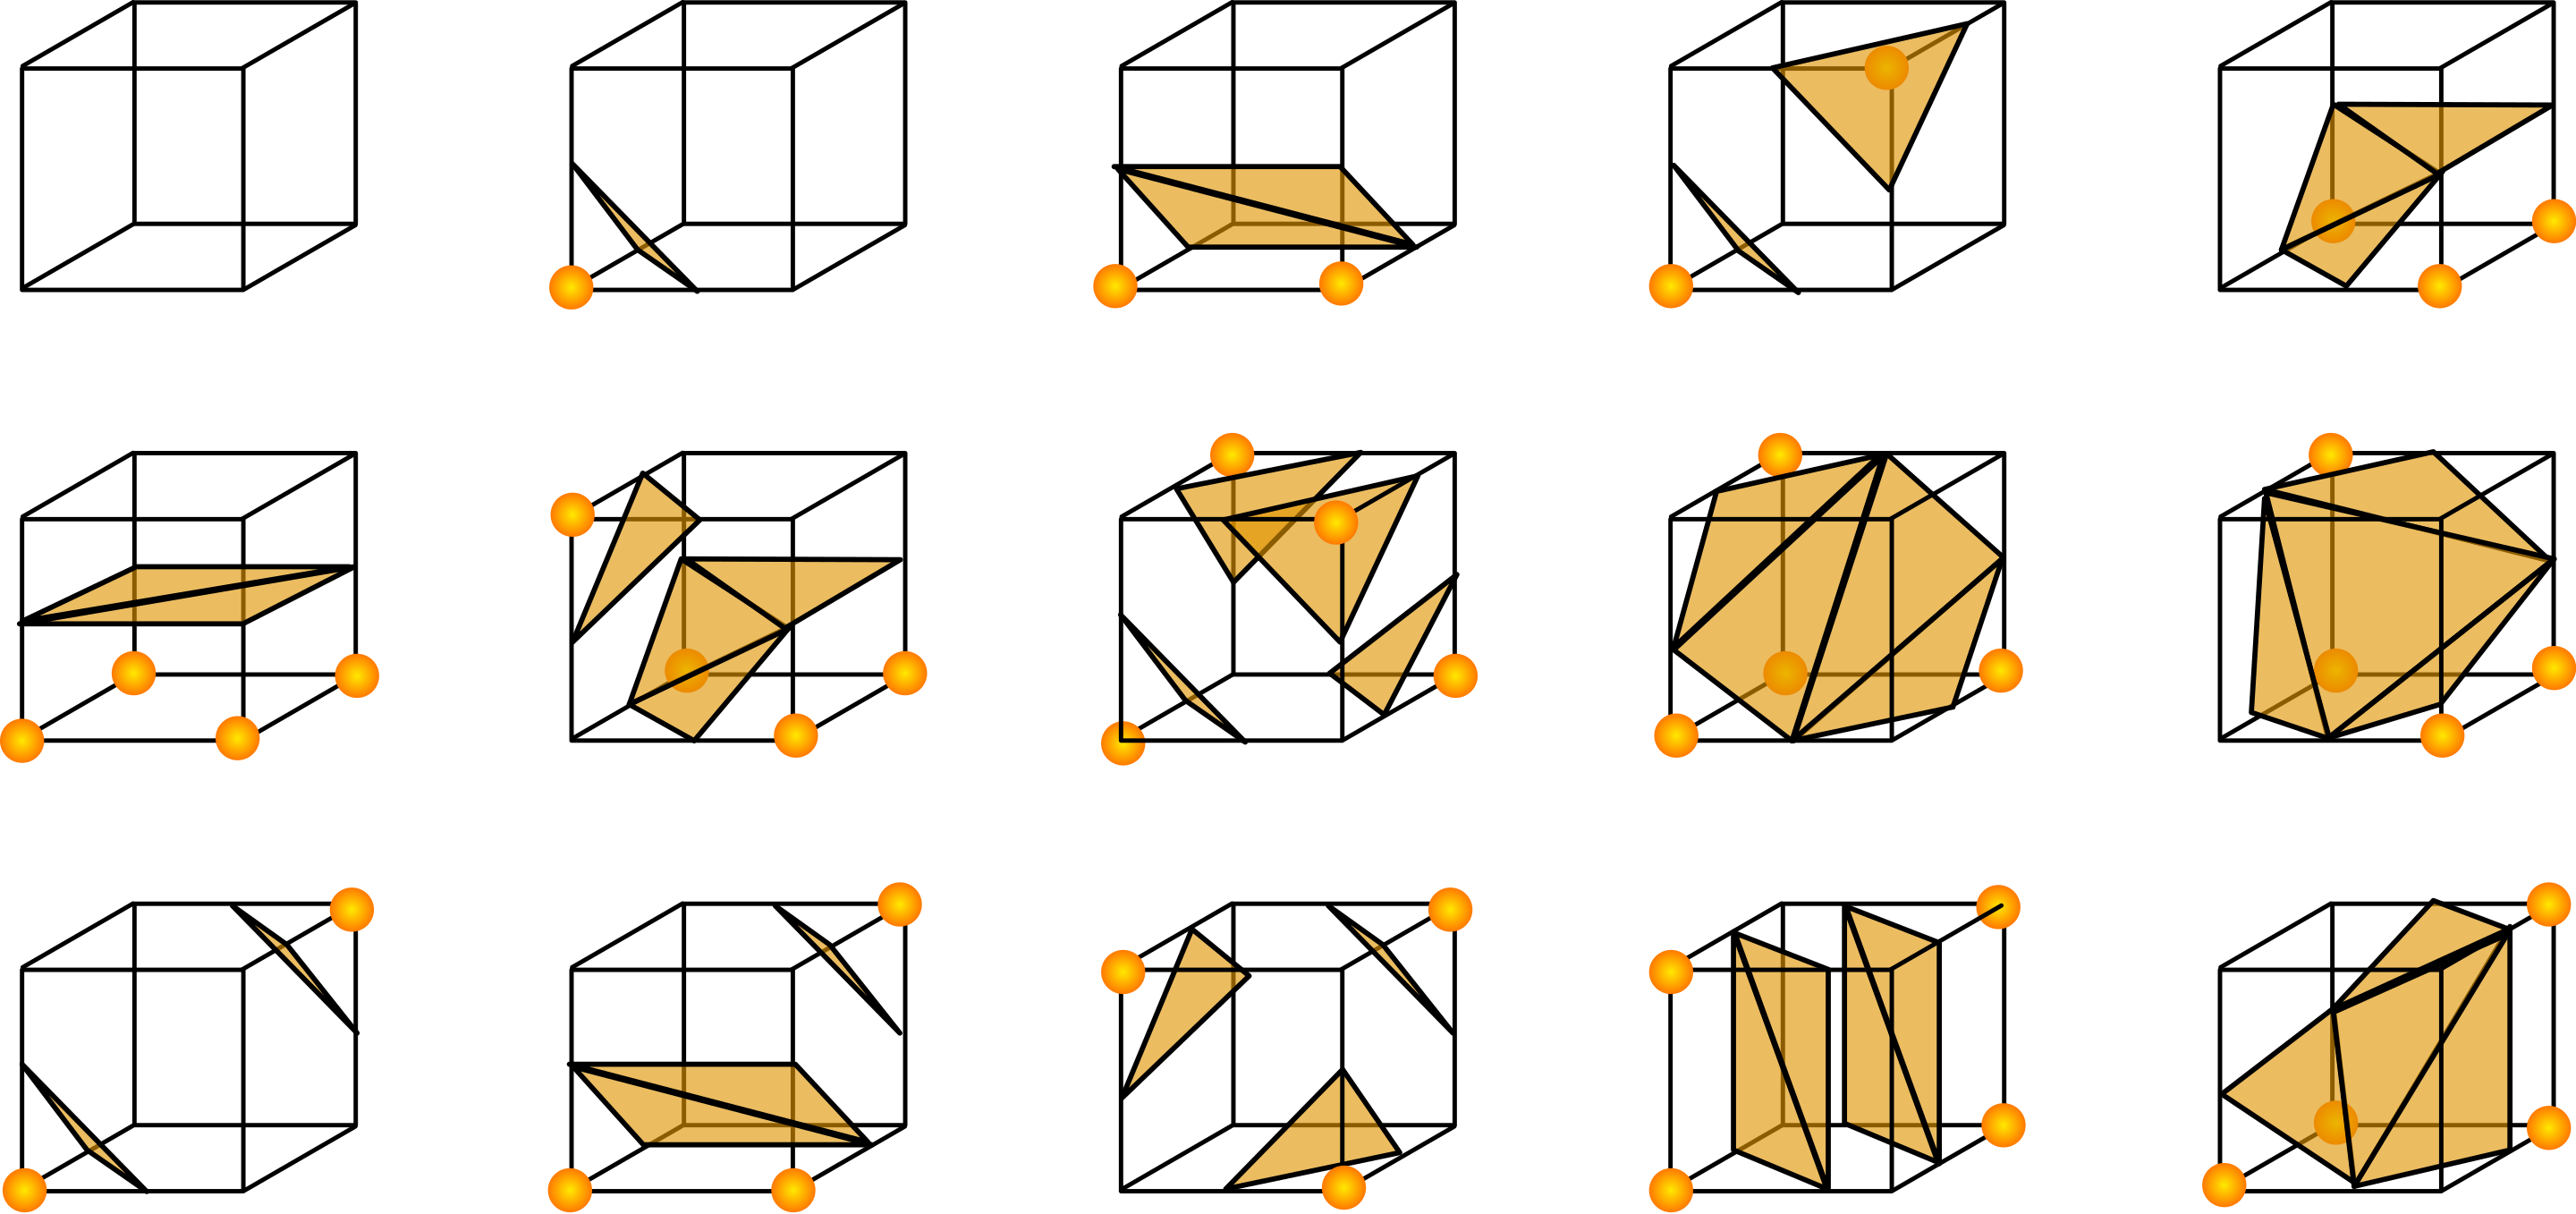
\includegraphics[width=\textwidth]{img/marching-cubes-config.png}
                    \caption{Marching cubes configurations \cite{wiki10}}
					\label{fig:marching-cubes-config}
				\end{minipage}
			\end{figure}
		
		\subsection{Smoothed Particle Hydrodynamic}
			Smoothed Particle Hydrodynamic (SPH) is a common computational method for simulating fluid flow on a machine. It was first published by Monaghan, Gingold and Lucy in 1977. In a SPH simulation, each fluid particle is interacting with its neighboring particle depending on its pressure, density, and velocity given a finite boundary around the particle. A particle's density is denoted as $$p_i=\sum_{j} m_jW_{ij}$$ where $W_{ij}$ can be any smoothing kernel. The pressure is then calculated with the ideal gas law in thermodynamics, written as $P=K(p-p_0)$. With the found density and pressure of a particle, we can find its acceleration by the following equation, $$a_i=-\sum_{j} \frac{m_j}{m_i}\frac{P_i+P_j}{2p_ip_j}\nabla W_{ij}\hat{r}_{ij}$$ where $\nabla W_{ij}$ is another smoothing kernel and $\hat{r}_{ij}$ is the normalized vector of a surrounding particle to the current particle. Finally, the particle position is being updated according to the computed acceleration. 

    \section{Implementation}

        We have used GLFW and GLSL. GLFW is a cross-platform utility library for creating window and OpenGL context, and we will use it for handling both window and input events. While GLFW handles all the high-level program logic, our project focuses on the low-level rendering. Mainly we will use GLFW to manage the OpenGL context. GLSL is the shading language for OpenGL which enables developers to control over the rendering pipeline. We will use GLSL to write our shader programs.
        
        The metaball positions are updated on the CPU, and sent to the GPU on every update frame. We send all data about the metaballs as a GLFW Texture2D object. For n balls, the texture has the size n by 1, and each pixel encodes that balls position as its RGB values, and the radius as its alpha value. This proved ideal. Since Texture2D objects can be sent multiple times with different sizes, we can dynamically set the metaball count and the positions of each particles. Furthermore, since the Texture2D is easily iterated through on the GPU by using a Sampler object, it was trivial to extract the ball position and radius from each pixel.

        To limit the pressure that the program puts on the CPU, we limited the CPU framterate to 60, by using a main loop that only runs the animation calculations and updates the GPU at fixed intervals.

        \subsection{Marching cubes}
        	\begin{minipage}{\linewidth}
			    \begin{lstlisting}
					private void Test(){
					int a = 1;
					}
				\end{lstlisting}
        	\end{minipage}
        
		\subsection{Smoothed Particles Hydrodynamic}
        \begin{minipage}{\linewidth}
        	\begin{lstlisting}
        	private void Test(){
        	int a = 1;
        	}
        	\end{lstlisting}
        \end{minipage}

        \subsection{Misc}
            For the purpose of creating a nice demo, we created a fragment shader with basic Phong illumination, in order to give the animation more depth.
            We also added a physics model to the balls which consists of outer forces due to gravity and a repelling force between each pair of balls when they are close to each other, to prevent them from accumulating in one place.
            We also modeled the bounciness of the floor and walls of our simulation domain, in order to keep the balls confined and in motion for as long as possible.

            We will not go into the details of how we implemented physics and the illumination model, as they are out of the focus of this report.

    \section{Result}
        Figure 4 shows three still images of our final rendering. 
        An animated video can be found here:
        \url{https://youtu.be/jmScNqchXs0}.

        Both the figure and the video show the same real time simlution, consisting of 100 particles and a voxel grid size of 80 units.
        The same physics and lightning models that were mentioned at the end of section 4 have both been applied.

        \begin{figure}[H]
        	\begin{minipage}[b]{0.5\textwidth}
	            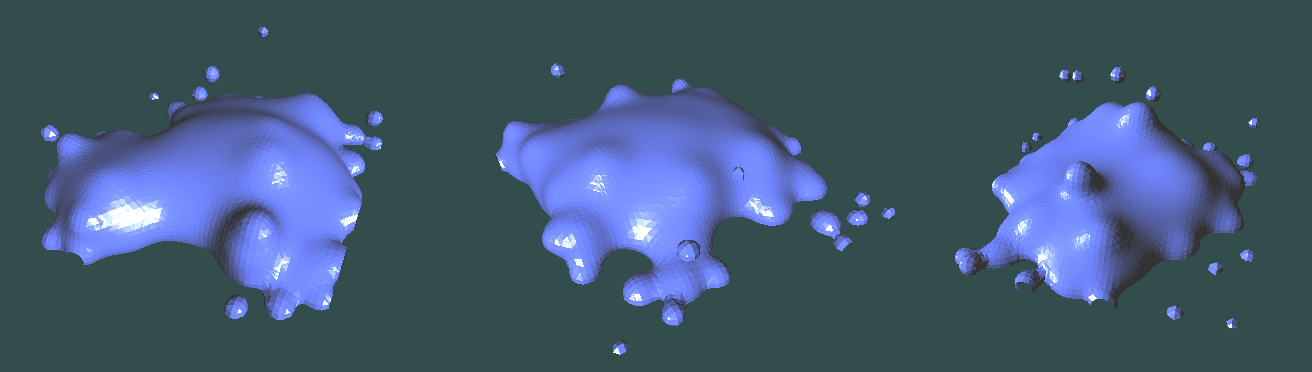
\includegraphics[width=\linewidth]{img/result-animation.png}
				\caption{Screenshot of the final animation, taken at fixed intervals. Note that the camera view is rotating around the model at a constant speed.}
				\label{fig:result-animation}
        	\end{minipage}
        \end{figure}

    \section{Conclusions}
    
        \subsection{Rendering model}
        
        One of our main obstacles with the simulation was that we could not run it with a high enough voxel grid count to render an impressive looking fluid on a large simulation domain.
        The cell count of the voxel grid is simply the resolution at which the fluid can be renderered.
        A high enough cell count will make the fluid appear smooth and seamless, but as the cell count decreases, the sharp edges of the mesh will become visible and the mesh as a whole will appear coarse and chunky.

        In order to find out wether the voxel shader or the particle model were the performance bottleneck, we ran a series of tests of the same simulation, with varying numbers of particles.
        The test was run on a NVIDIA Geforce GTX 1050 Ti.
        For each test we noted the maximum voxel cell count we could use while still running the simulation reliably above 30 frames per second.
        The following table lists the mumber of metaballs vs the maximum voxel grid cell count we could use before the framerate would drop below 30 fps:

        \begin{tabular}{ l | c | r }
          50 & 120 \\
          20 & 160 \\
          5 & 200 \\
        \end{tabular}

        Finally: disabling the metaball filter completely, and just running the voxel shader itself, yielded a maximum voxel cell count of 310 units before the framrate dropped below 30.
        Our conclusion is that the geometry shader itself, without any particles, can run with a voxel grid size in the order of 100-200 units at 60 fps, and up to 300 units at 30 fps.
        For our purpose, this can be used to create a nice looking dynamic fluid on a small simulation domain, or a very chunky looking fluid on a medium sized to large sized simulation domain, or a fluid with very few particles.
        To render an impressive fluid in a medium sized voxel grid, it would be nice if we could optimize the particle model so that we could run in the order of 100 particles at a voxel grid size of 200.
        The following section about the particle model will discuss some ideas for how this could be achieved in theory.

        \subsection{Particle model}
        It seems that the industry standard for fluid simulation in high quality games and video is the Smoothed Particle Hydrodynamics (SPH) model with Ellipsoid Splatting rendering.
        The SPH model uses nearest neighbour search to find out how a particle should collide.
        Ryan L. Guy presented his SPH implementation in a paper for the University of Virginia. He profiled his simulation times, and from the results we can see that the majority of the simulation time (around 75\%-85\%) is spent in the nearest neighbour search.
        Thus the goal for the particle model must be to optimize the nearest neighbour search for all particles.
        Guy has done this by implementing a spatial grid that functions as a lookup table for the particles.
        Any particle will begin its nearest neighbour search in the grid cell in which it is contained, and continues to search through the nearest 26 cells until the nearest neighbour is found.
        The fixed grid size was set to the one smoothing radius of the particle system, which is the maximum distance at which any two particles will interact.
        \cite{guy15}

        In comparison with our implementation, currently we are very much brute forcing when calculating the potential field over all particles.
        For each voxel grid cell, all particles and their influences on that point are taken into account, even if they are so far away that their contribution of the field is negligable.
        We can however use Guy's idea of spatial subdivision, by assigning the particles to their own grid cells, to detemine which range of particles should realistically have influence over a given point, before iterating through them 
        We imagine implementing this as a spatial structure that is embedded in the texture that sends the particle positions to the GPU.
        Each Y-cooridate of the texture could represent a grid cell, and all pixels on that column would still represent the particles that are in that cell, their positions and sizes.
        Even after transforming the 3D grid to a linear structure one could simply define a lookup function that continues the nearest neighbour search in the neighbouring cells, and terminating after a certain depth if no neighbour particles are found.
        We could very well experiment with different values of the smoothing radius and thus the fixed grid size, but a good initial guess might be the radius from a particle center at which the potential field evaluates to some low threshold, let us say 0.01. 
        This form of spatial subdivision would allow for more particles in the simulation, but since the voxel shader itself cannot run reliably with a grid size above 200-300 units, it would not yield the neccessary performance increase that is needed to simulate particles in a high-resolution domain.

        Yet another performance problem comes from the fact that the division step in our metaball potential function is computationally expensive.
        Ryan Geiss (whose tutorial on the metaball isosurface model we used for this project) came with a suggestion for an approximate polynomial function which should in theory be faster on the GPU. His suggested function was:

        \begin{center}
        $[g(r) = r^4 - r^2 + 0.25]$
        \end{center}

        This potential field function also has the neat property that it evaluates to 0 at $r=\frac{1}{\sqrt{2}}$, which means that you could do spatial optimization by only evaulating the points that fall within the radius of $r=\frac{1}{\sqrt{2}}$ of a singe metaball's center.
        \cite{geiss00}

        Our prediction is that this would yield a similar performance increase to implementing a naive spacial subdivision, but we are still not solving the problem that the voxel shader itself is expensive.
        To address this, our suggestion would be to redo the rendering model and instead use a point-based or ellipsoid-based splatting rendering method, which would be much more ideal for real time fluid simulation.

	\end{multicols}

\begin{thebibliography}{9}

\bibitem{geiss00}
  Ryan Geiss,
  \textit{Metaballs (also known as: Blobs)},
  October,
  2000.
  \\
  http://www.geisswerks.com/ryan/BLOBS/blobs.html

\bibitem{heckbert92}
  Paul Heckbert,
  \textit{Intro to Metaballs},
  November,
  1992.
  \\
  https://steve.hollasch.net/cgindex/misc/metaballs.html


\bibitem{guy15}
  Ryan Guy,
  \textit{Smoothed Particle Hydrodynamics Fluid Simulation},
  2015.
  \\
  http://rlguy.com/sphfluidsim/

\bibitem{wiki07}
  Image from: https://en.wikipedia.org/wiki/File:Metaballs.png

\bibitem{wiki10}
  Image from: https://en.wikipedia.org/wiki/File:MarchingCubes.svg

\end{thebibliography}

\end{document}
